\section{Errata for the base paper}
\label{sec:errata}

We read the base report~\cite{garlapati2026ecm} closely and re-derived or re-implemented what could be checked without the authors' code.
Table~\ref{tab:errata} lists what we found; the script \texttt{experiments/e0\_errata\_checks.py} reproduces every number quoted in this section.
We separate items we verified (analytically or numerically) from concerns that need the original code to quantify.
None of this detracts from the report's candour: several items below sharpen negative results that it already states.

\begin{table*}[p]
\centering
\caption{Errata. Status: \textbf{A}~shown analytically, \textbf{N}~verified numerically here, \textbf{T}~follows from the base paper's own text or tables, \textbf{C}~concern that needs the authors' code to quantify.}
\label{tab:errata}
\footnotesize
\setlength{\tabcolsep}{4pt}
\renewcommand{\arraystretch}{0.96}
\begin{tabular}{@{}r p{0.095\textwidth} p{0.30\textwidth} p{0.475\textwidth} l@{}}
\toprule
 & Where & Statement or practice & Finding & \\
\midrule
\multicolumn{5}{@{}l}{\emph{Permanence score (PVS)}}\\
1 & Eq.~3 & ``Motion explained by noise alone costs nothing.'' & False. The clamp at zero leaves $\mathbb{E}[s]=1/(e\ln 2)=\NullBias$ bits/px under the paper's own Laplacian noise model ($2^{-\delta}$ times that with dead zone $\delta$). & A, N\\
2 & Eq.~3 vs.\ Eq.~2 & Eq.~3 is called the Lagrangian form of the balance law. & It is not. The Lagrangian form of Eq.~2 concerns the scalar density, which the paper shows fails (0.57 AUC). Eq.~3 is a noise-normalised motion-compensated residual, i.e.\ warping error in other units; only the mask comes from the balance law. & A\\
3 & Eq.~3--4 & PVS is read as a share of the frame's information. & Eq.~3 charges a pixel without bound, so PVS is not a fraction (the paper itself reports 2.22). A legal soft spotlight scores $\SpotPVS$ under the paper's $\sigma{=}2$ prefilter, with single pixels charged $\SpotPeak$ bits; capping by the intra cost gives $\SpotCapped$. & N, T\\
4 & Eq.~3--4 & One threshold for all footage. & Numerator is relative to the clip's noise, denominator is absolute bits: one fixed event scores $\NoiseA$, $\NoiseB$, $\NoiseC$ at noise $\sigma=3,\,1.5,\,0.75$ grey levels. Clean (generated, denoised, blurred) footage is scored far more harshly than grainy footage. & N\\
5 & \S4, \S4.3 & Clip score is $\max_t\mathrm{PVS}_t$. & Grows with clip length. Two event-free sets with 127 and 15 frame pairs are separated with AUC $T_1/(T_1{+}T_2)=\LenAUC$. The synthetic and real clips differ in length. & A, N\\
6 & \S4.3 & ``There was no separation'' (real vs.\ generated). & 4 real and 15 generated clips, no violation labels, mixed lengths and noise levels (items 4, 5): the test can show neither separation nor its absence. \S7 calls it ``19 clips''. & T\\
7 & Table~1 & AUC differences of 0.01--0.03 are interpreted. & No uncertainty is reported. With about 150 clips per class the standard error of an AUC near 0.8 is about 0.026. & A\\
8 & \S4.1--4.2 & Headline 0.86 (clean) and 0.80 (stress). & As far as the text specifies, the two use different pipelines (prefilter off / on); no single configuration is reported on both sets. & C\\
9 & \S4.2 & Occlusion boundaries from the neighbouring frame pairs. & Fixes one-frame events only. A melt, fade or boil spans the neighbouring pairs as well, so the spurious boundaries return. & C\\
10 & \S3--4 & Sources are legal at occlusion boundaries. & \emph{Any} creation there is free: an object that changes identity behind an occluder, or never re-emerges, costs nothing. The balance law has no storage term. & A\\
\midrule
\multicolumn{5}{@{}l}{\emph{Frame-shared generation}}\\
11 & Eq.~5 & Proportional attention ``reproduces full attention exactly''. & Only without temporal position information, which a video model needs. Random transformer: relative error \PropExact{} without a temporal embedding, $\PropPE$ with one. The paper's own oracle result (43.6\,dB, falling as more frames share) is not exact either. & N, T\\
12 & Table~2, Fig.~4 & Sharing ``lies clearly above the fewer-steps baseline'' (41.5--43.8\,dB vs.\ 27--30\,dB). & Different references. Baselines are scored against the original output; sharing is scored against full compute from noise the method has already tied. Against the original, sharing scores 11--15\,dB (\S5 of the paper), below every baseline in the table. & T, N\\
13 & \S5 & Whether the shared-noise sample is as good is ``untested''. & It has an answer: copying one frame's noise to $F$ frames is not distribution-preserving. Static content is driven by noise $\sqrt F$ too strong (Theorem~\ref{thm:copy}). & A, N\\
14 & \S5 & Static map from a 2-step draft. & The draft runs on independent noise, the final sample on tied noise 11--15\,dB away. The map describes a video that is never generated. & T\\
15 & \S5 & 41.5--43.8\,dB fidelity. & Finer than the reference itself: 20 and 40 steps differ by 39.2\,dB. Above about 39\,dB the metric measures agreement with a discretisation error. & T\\
16 & Table~2 & Projected speedups 3.7--5.7$\times$. & Include a fixed draft cost of 2 of 20 full steps. At the 90\,\% setting the draft is \DraftShare\,\% of the projected cost, and it caps any speedup at 10$\times$. (Our FLOP model reproduces the projections: \ProjLo$\times$ and \ProjHi$\times$.) & A\\
17 & \S5 & Static tokens settle earlier, taken as support for the temperature view. & Predicted by pooling alone (Eq.~\ref{eq:clock}), with no role for information density. & A\\
\bottomrule
\end{tabular}
\end{table*}

\paragraph{The score charges noise (item 1).}
For a Laplacian residual with scale $b$, $u=|r|/b$ is exponential with unit rate and Eq.~3 reads $s=\max(u-1,0)/\ln 2$.
Before the clamp its mean is zero, which is the property the paper states.
After the clamp it is $\int_1^\infty(u-1)e^{-u}du/\ln 2=1/(e\ln 2)=\NullBias$ bits per pixel.
At the 3.6--4.2 bits/px the paper quotes for its clips this alone implies $\mathrm{PVS}_t\approx\PvsFloor$ for a clip in which nothing happens, twenty to forty times the 0.003--0.007 shown for legal clips in its Fig.~1.
Our re-implementation of Eqs.~1, 3 and 4 gives $\SpotNoEvent$ for an event-free noisy scene, as predicted.
The printed equations therefore do not determine the printed numbers.
The likely reason is that the synthetic clips are noise-free, so the residual is exactly zero on the static background; but then $b=\mathrm{median}|r|/\ln 2=0$ and Eq.~3 is undefined without a floor that the paper does not report.

\paragraph{The score is not a fraction, and depends on grain (items 3--4).}
Eq.~3 is linear in $|r|$ with slope $1/(b\ln 2)$ bits per grey level, however small $b$ is.
A code can always fall back to sending the pixel without reference to the previous frame, so a consistent ``created information'' is at most the intra cost $\iota$ of the new pixel.
Without that cap, cleaner footage is charged more for the same change (Fig.~\ref{fig:errata}c).
This is a confound for the real-versus-generated test, where one class has camera grain and the other does not, and it matches the paper's remark that compression doubled the peak score for identical content.

\paragraph{The headline fidelity uses a moved reference (item 12).}
This is the most consequential item and the starting point of our own work.
The $\dagger$ footnote of the base paper's Table~2 states the reference honestly, but the comparison drawn from it in Fig.~4 does not hold.
The tied-noise reference also rewards over-sharing: marking more positions static pulls the reference and the output towards the same frozen video, so the metric cannot see the method's main failure mode.
We reproduce both numbers in \S\ref{sec:trained}: copy-tied sharing agrees with its own tied reference to $\ACopyOwnRef$\,dB and with the original sample to $\ACopyOrig$\,dB.

\begin{figure*}[t]
\centering
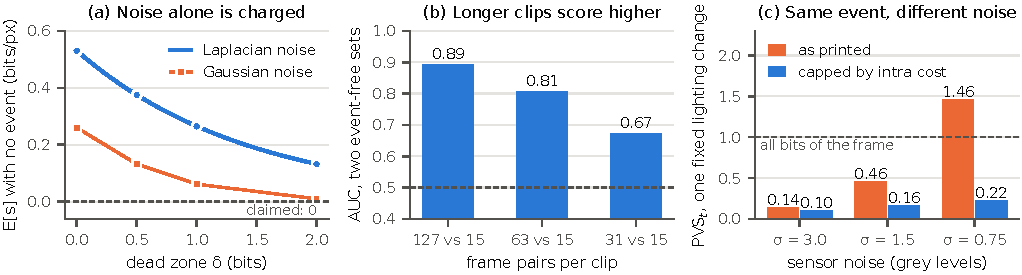
\includegraphics[width=\textwidth]{../figures/fig_errata.pdf}
\caption{Three of the errata, checked numerically. (a)~Expected value of Eq.~3 when the residual is pure noise; the base paper states it is zero. (b)~AUC between two sets of clips that contain no event and differ only in length (dashed: no bias). (c)~PVS$_t$ of one fixed legal lighting change under three noise levels, as printed and with the per-pixel charge capped by the intra cost.}
\label{fig:errata}
\end{figure*}
